\section{Основные результаты наблюдений} % (fold)
\label{sec:ObservationResults}
	Поскольку экспериментальное наблюдение стадных явлений не является темой данной работы, мы не будем останавливаться подробно на результатах полевых или лабораторных исследованиях, тем более что всестороннее освещение этого вопроса дано в работе Вичека~\cite{vicsek2012}. Однако для лучшего понимания распространенности в природе стадных явлений будет приведен краткий обзор наиболее характерных, с нашей точки зрения, работ, сгруппированных по исследуемому материалу. Итак, в разные годы обьектами исследования становились:
	\begin{enumerate}
		\item Внутриклеточные соединения~\cite{chowdhury2006,keller1971}
		\item Колонии бактерий~\cite{czirok1998,csahok1997}
		\item Насекомые~\cite{buhl2006}
		\item Птицы~\cite{ballerini2008,selous1931,dellariccia2008,biro2006,major1978,nagy2010}
		\item Рыбы~\cite{cambui2012,makris2009,parrish1997}
		\item Млекопитающие, к примеру, буйволы~\cite{sinclair1977}
	\end{enumerate}
	Особняком в этом ряду стоят наблюдения за океаническим планктоном~\cite{seuront2004} и превышающие по своей численности наблюдения за любым другим типом обьектов, наблюдения за поведением групп людей, например~\cite{parisi2009,moussaid2011}.

	Кроме того, в совершенно отдельную группу необходимо выделить лабораторные эксперименты, проводимые с неживыми обьектами --- нематической жидкостью, колеблющимися металлическими стержнями, наночастицами в жидкости, микророботами и тому подобным.~\cite{schaller2010,turgut2008,blair2003}

	Теперь приведем основные результаты, полученные в ходе наблюдений. Для начала, необходимо четко разделять работы, в которых исследования велись на плоскости (все, кроме указанных далее) и в которых наблюдения велись в трехмерном пространстве~\cite{cullen1965,ballerini2008,major1978,makris2009}. Хотя, как выяснилось, для рыб такое разделение не вполне необходимо. Но обо всем по порядку.

	Главный вывод, который в общем-то и не нуждается в подтверждении --- это то, что существует отдельный класс перемещений группы индивидов как целого, и при этом перемещения отдельных индивидов оказываются упорядочены. То есть, при определенных условиях (чаще всего рассматривается различная плотность на единицу площади, или обеспеченность ресурсами в широком смысле слова) происходит спонтанное нарушение симметрии, и хаотическое движение сменяется упорядоченным. Как уже говорилось, это наблюдается на всех масштабах природы, и более того --- совершенно не обязательно при этом прямое (визуальное или тактильное) взаимодействие между особями, и бывает достаточно опосредствованного взаимодействия через среду обитания~\cite[с. 119]{vicsek2012}. %добавить информацию про молекулы, перекидывающие взаимодействие через жидкость в которой они живут
	Следующее наблюдение на которое указывают многие авторы: при нарушении симметрии возникает и дальний порядок связи, к примеру, рыбы могут изменять общее направление движения практически мгновенно~\cite{cambui2012}, а птицы --- так-же быстро принимать решения о посадке.~\cite{lukeman2010,major1978}.

	более того, самым удивительным явлется то, что у всех живых существ и неживых предметов, при движении которых проявляются стадные явления, качественный характер этих явлений практически одинаков. %(Не считая сугубо трехмерных формаций, которые образуются в стаях птиц, однако и там можно выделить правильный ``параметр порядка'').
	\begin{figure}
        \centering
        \begin{subfigure}{.4\columnwidth}
                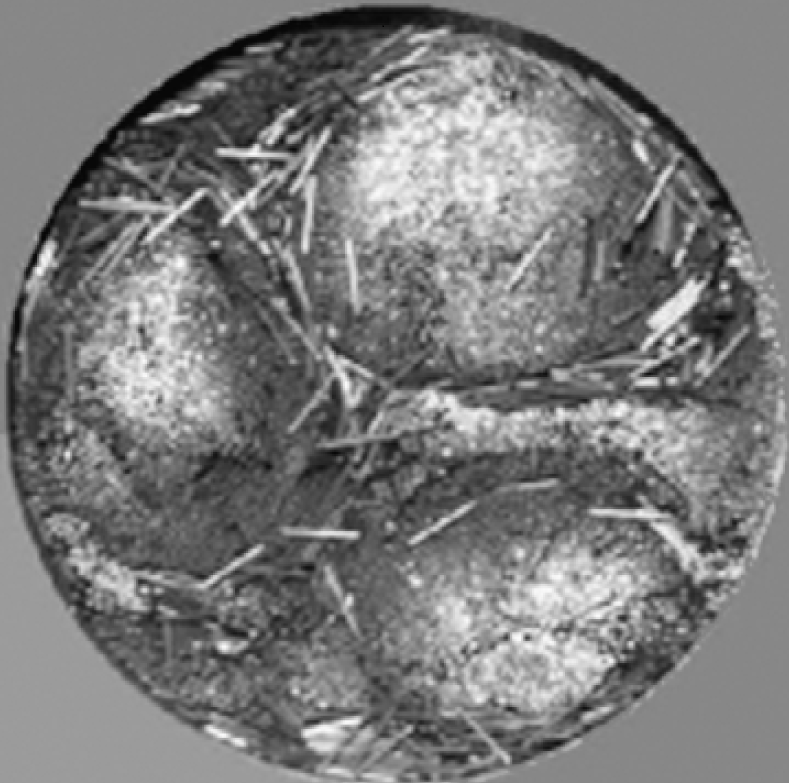
\includegraphics[width=\columnwidth]{Images/Fig4_CollectiveMotion.png}
                \caption{A nematics}
                \label{fig:CollMot:nematics}
        \end{subfigure}%
        ~ %add desired spacing between images, e. g. ~, \quad, \qquad, \hfill etc.
          %(or a blank line to force the subfigure onto a new line)
        \begin{subfigure}{.4\columnwidth}
                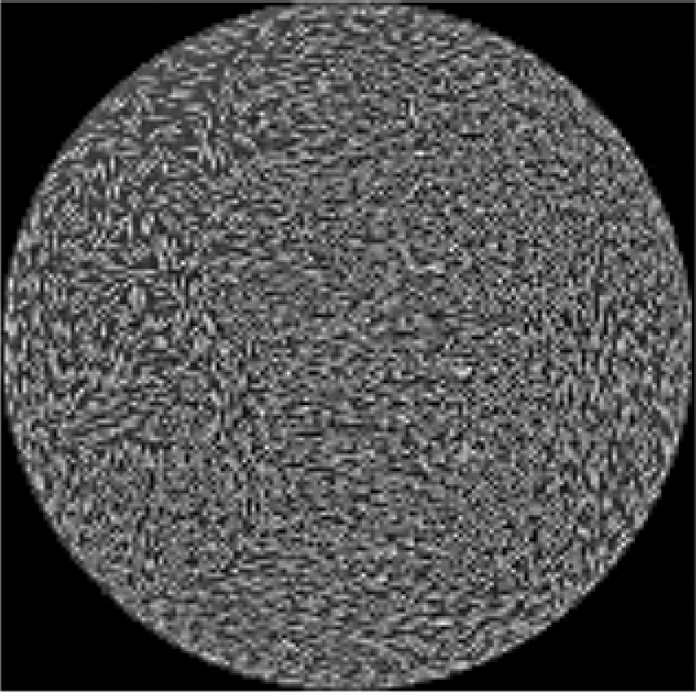
\includegraphics[width=\columnwidth]{Images/Fig6_CollectiveMotion}
                \caption{A rods on wibe}
                \label{fig:CollMot:rods}
        \end{subfigure}
        \caption{Упорядочивание неживых обьектов}
        \label{fig:CollMot:NonLiving}
    \end{figure}
        ~ %add desired spacing between images, e. g. ~, \quad, \qquad, \hfill etc.
          %(or a blank line to force the subfigure onto a new line)
    \begin{figure}
    	\centering
        \begin{subfigure}{0.3\textwidth}
                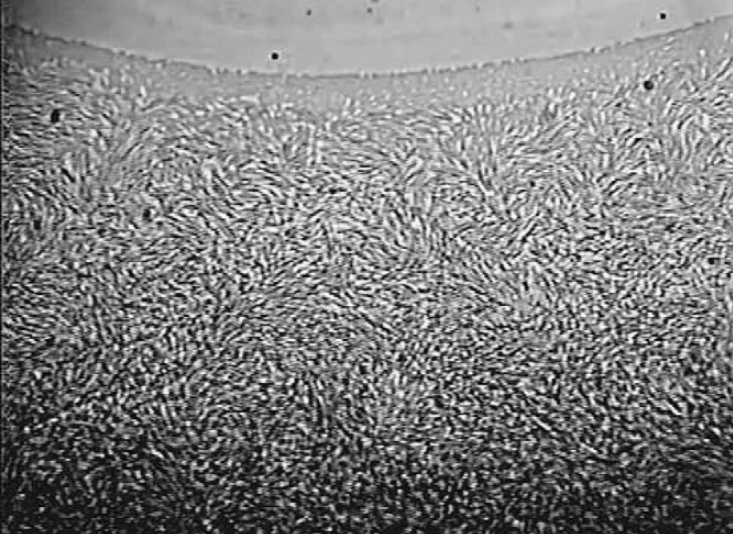
\includegraphics[width=\textwidth]{Images/Fig11_CollectiveMotion}
                \caption{A bacteria 1}
                \label{fig:CollMot:bacteria}
        \end{subfigure}
        \begin{subfigure}{0.5\textwidth}
                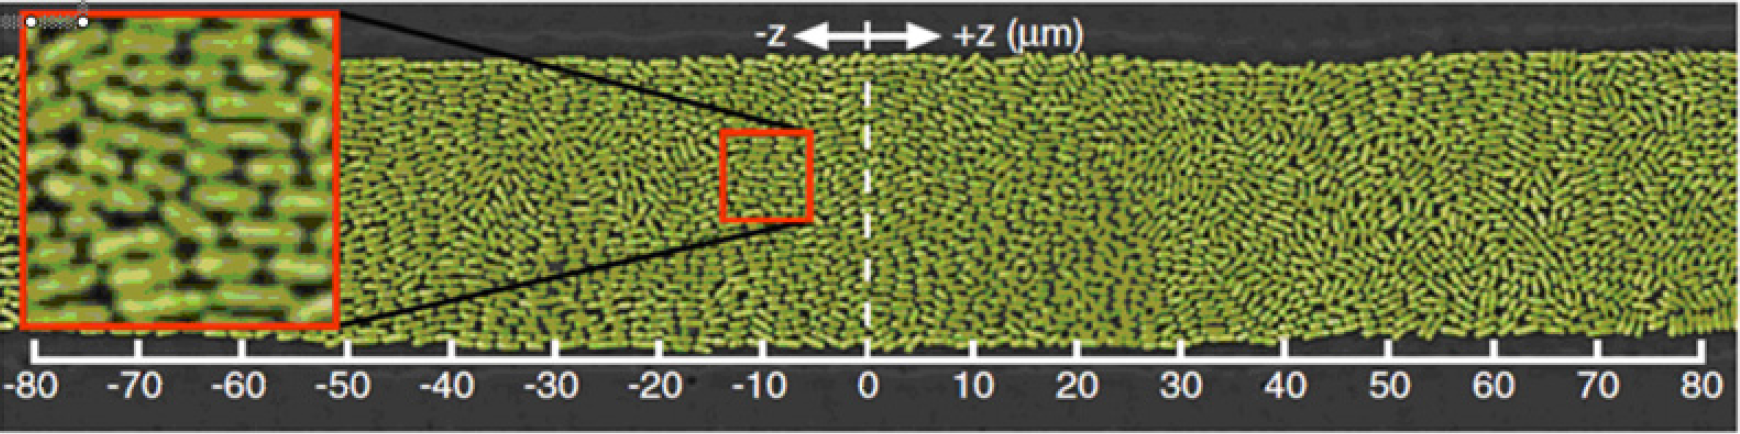
\includegraphics[width=\textwidth]{Images/Fig15_CollectiveMotion_part}
                \caption{A moleculae}
                \label{fig:CollMot:moleculae}
        \end{subfigure}
        \caption{Микроскопические проявления групповой динамики}
        \label{fig:CollMot:microscpoic}
    \end{figure}
    \begin{figure}
    	\centering
        \begin{subfigure}{0.4\textwidth}
                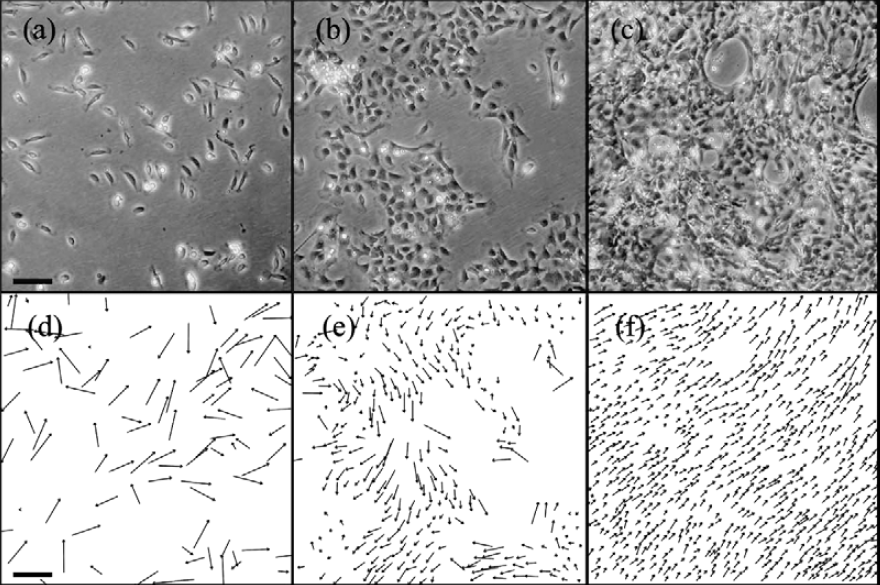
\includegraphics[width=\textwidth]{Images/Fig17_CollectiveMotion}
                \caption{A fishes}
                \label{fig:CollMot:fishes}
        \end{subfigure}
        \begin{subfigure}{0.4\textwidth}
                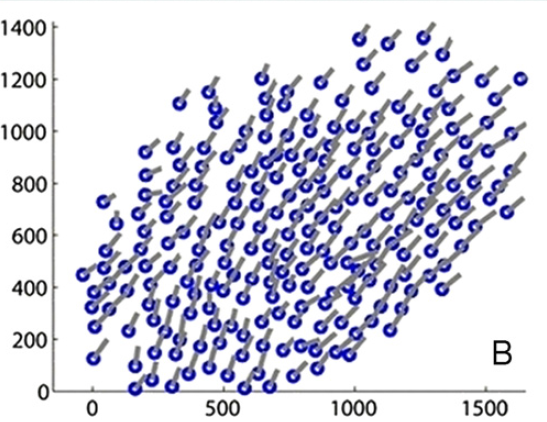
\includegraphics[width=\textwidth]{Images/Fig29_CollectiveMotion_part}
                \caption{A ducks}
                \label{fig:CollMot:ducks}
        \end{subfigure}
        \caption{Макроскопические проявления группового движения}\label{fig:CollMot:macroscopic}
	\end{figure}

	Наглядно это можно рассмотреть на рис. \ref{fig:CollMot:NonLiving}, \ref{fig:CollMot:microscpoic}, \ref{fig:CollMot:macroscopic}. Особенностью всех представленных на изображениях обьединений является то, что они расположены на плоскости. И, как мы видим, возникает два типа упорядоченностей, иногда (как на рис. \ref{fig:CollMot:nematics}) проявляющихся единовременно: это упорядоченное движение в спонтанно выбранном направлении или упорядоченное обращение вокруг некоторого центра. Видно также, что для совершенно, казалось бы, различных обьектов групповое поведение является очень схожим.

	Что же касается перемещений, не ограниченных в двух плоскостях, то нам хотелось бы заострить внимание на трех моментах. 

	Во-первых, в обьемном пространстве также наблюдаются все вышеперечисленные упорядоченные перемещения: птицы сбиваются в стаю и летят в выбранном направлении~\cite{dellariccia2008}, насекомые кружат вокруг улья~\cite{buhl2006} и т.п.

	\begin{wrapfigure}{r}{0.5\textwidth}
	  \vspace{-20pt}
	  \begin{center}
	    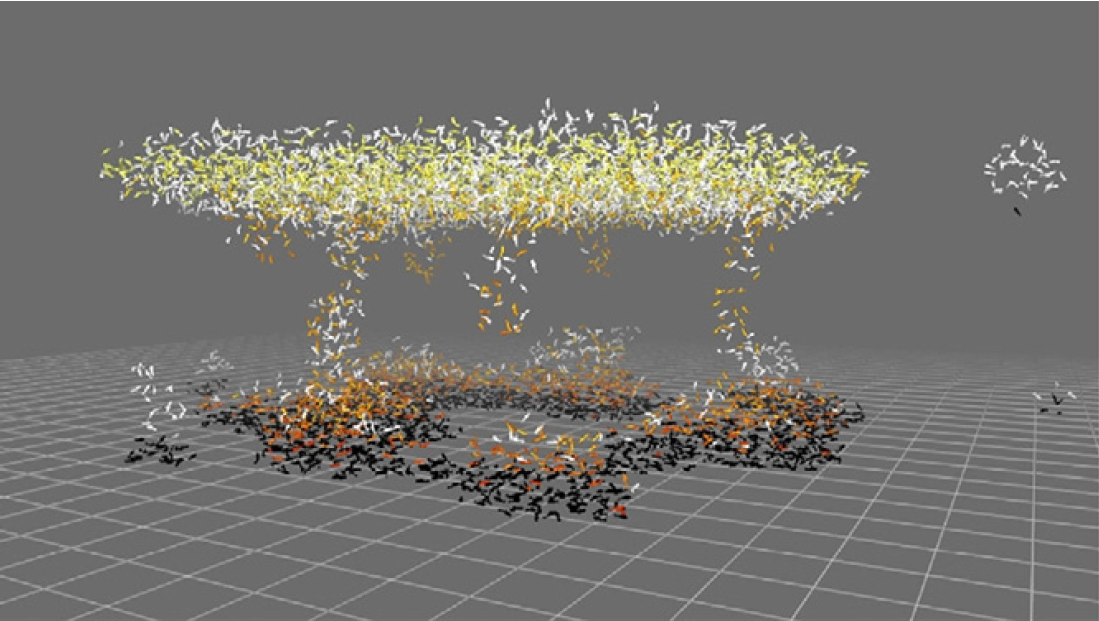
\includegraphics[width=0.48\textwidth]{Images/Fig57_CollectiveMotion}
	  \end{center}
	  \vspace{-20pt}
	  \caption{Расслоение косяка рыб}
	  \label{fig:FishSplitting}
	  \vspace{-10pt}
	\end{wrapfigure}

	Во-вторых, и это является особенностью косяков рыб, возможно расслоение трехмерной группы на более плоские подгруппы, с наличием соединяющих (цилиндрических) столбов. Предполагается, что это это связано с ``мотивацией'', например, молодая стерлядь во время нереста предпочитает подниматься выше, а более старая опускается вниз.~\cite{axelsen2000} При этом наблюдаются структуры подобные изображенным на рис. \ref{fig:FishSplitting}

    \textcolor{red}{В дальнейшем в этой части можно указать что в групповых явлениях наблюдаются ``лидеры'', которые могут задавать движение. Еще где-то надо сказать что фазовый переход переходит или при уменьшении шума, или при увеличении плотности, наверно в следующем пункте}

% subsection основные_результаты_наблюдений_за_системами_демонстрирующими_группувую_динамику (end)